\documentclass[12pt, a4paper]{article}
\usepackage[utf8]{inputenc}
\usepackage[ngerman]{babel}
\usepackage{csquotes}
\usepackage{listings}
\usepackage{amsmath}
\usepackage[ngerman]{struktex}
\usepackage[backend=biber,dateabbrev=false, sorting=none]{biblatex}
\usepackage{forest}
\usepackage{graphicx}

\lstset{language=Python}

\addbibresource{wpa.bib}
\graphicspath{ {./img/} }

\title{\textbf{Emotionserkennung mit künstlichen neuronalen Netzen}\\ {\normalsize wissenschaftlich-praktische Arbeit}}
\author{Gustav Lahmann}
\date{8. Juni 2018}

\begin{document}

\begin{titlepage}
\maketitle
\centering
\small{\textit{Georg Cantor Gymnasium Halle (Saale)}}

\bigskip
\bigskip
\normalsize{Betreut durch: Herr Dipl.-Ing. (FH) Dirk Hesselbach}
\small{\textit{(Hochschule Merseburg)}}
% hide page number
\thispagestyle{empty}
\end{titlepage}


\tableofcontents
% hide page number
\thispagestyle{empty}
\newpage
\setcounter{page}{3}
\section{Einleitung}

Während der Arbeit in einer AG mit dem Thema künstliche Blumen bauten und programmierten die Mitglieder einen Kaktusroboter. Dabei entstand die Idee, dass er auf die Emotionen der Menschen in seiner Umgebung reagieren soll. Dieses Vorhaben wurde als Thema der wissenschaftlich Praktischen Arbeit aufgegriffen.

\subsection{Zielsetzung}

Das Ziel dieser Arbeit ist die Emotionserkennung in Gesichtern aus Bildern mit Hilfe von künstlichen neuronalen Netzen (KNN). Im aufgenommenen Kamerabild sollen Gesichter gefunden und anschließend jeder der Emotionen \textit{fröhlich}, \textit{traurig}, \textit{überrascht}, \textit{zornig}, \textit{angewidert}, \textit{verachtend} und \textit{ängstlich} ein Score zugeordnet werden, der angibt, mit welchem Anteil die jeweilige Emotion im Gesicht erkannt wurde. Der größte Score einspricht dabei immer der Emotion, die im Bild hauptsächlich vorliegt. Diese Emotionen entsprechen den Basisemotionen nach Paul Ekman und werden kulturübergreifend verstanden.\cite{wikipedia:facs} Da das KNN mit einer festen Zuordnung einer der oben genannten Emotionen zu jedem Beispielbild trainiert wird, muss diese Hauptemotion nicht immer der tatsächlichen entsprechen, da diese eine Kombination aus mehreren sein kann.

\subsection{Verwendung}
Unternehmen wie Affectiva nutzen die Emotionen des Nutzers um die Wirkung von Werbespots und Computerspielen zu beurteilen oder Stresssituationen beim Autofahren zu erkennen.\cite{affectiva:web}
Weitere Anwendungen sind die Windows Fotogalerie oder Snapchat Filter. In der Auswertung von Daten aus Überwachungssystemen zur Erkennung von Konflikten oder in Tests zur Benutzerfreundlichkeit von Software ist eine Verwendung ebenfalls denkbar.

\begin{figure}
	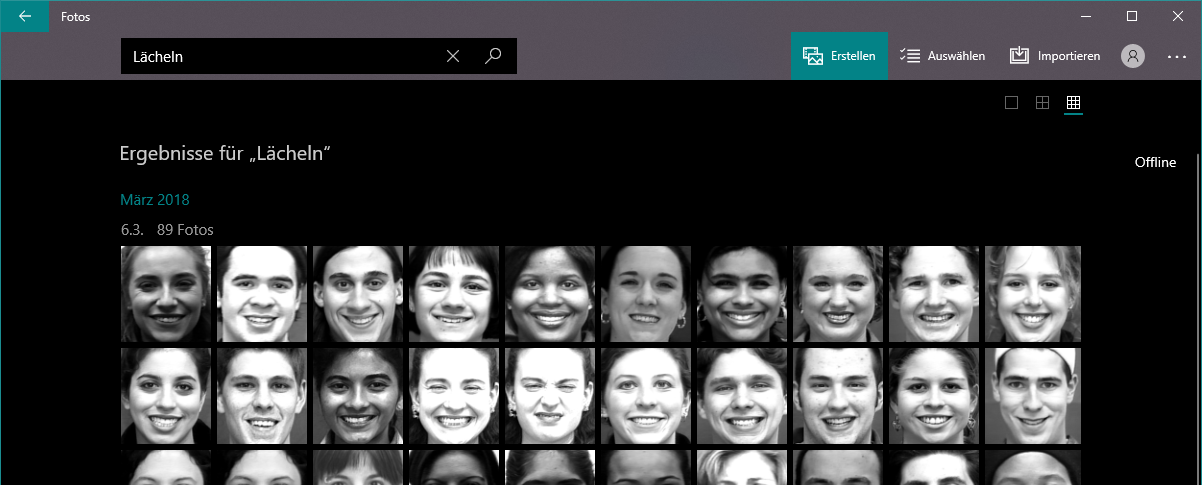
\includegraphics[width=\textwidth]{windows_fotos_laecheln_all_faces_top}
	\caption{Die Windows 10 Fotogalerie erkennt lächelnde Gesichter aus meinen Test- und Trainingsdaten und fasst sie in einem Album zusammen}
\end{figure}

\section{Vom Problem zum Programm}
Ziel ist es, ein alleinstehendes  Modul zur Emotionserkennung zu schaffen. Es kann später in den Roboter intrigiert werden und die Ergebnisse an andere Mikrorechner im System weiterleiten.

\subsection{Problemanalyse}

Das eingebettete System besteht aus einem Hardware und Software Teil. Als Erstes wird über eine Kamera ein Bild aufgenommen und an die Software übertragen. Diese wertet das Bild aus und erkennt zunächst mit Hilfe von Haar Features Gesichter im Bild. Anschließend wird das statistisches Auswertungsverfahren "Local Binary Pattern" (LBP) angewendet und die erhaltenen Häufigkeiten als Input für das KNN verwendet. Es wurde mit vorher klassifizierten Testbildern trainiert und erkennt die Emotion. Das Ergebnis wird anschließend grafisch als Balkendiagramm auf einem Display ausgegeben.

\bigskip
\begin{forest}
[{Eingebettetes System} 
	[Hardware
		[Eingabe [Kamera]] 
		[Verarbeitung [Mikrorechner]] 
		[Ausgabe [Bildschirm]] 
	] 
	[Software 
		[Gesichtserkennung [Haar Features]]
		[Emotionserkennung
			[LBP]
			[KNN]
		]
	]
]
\end{forest}


\subsection{Technische Basis}
Das möglichst minimal gehaltene System, welches verwendet wurde, besteht aus einem \textit{Raspberry Pi 3 Model B} (64bit QuadCore CPU mit 1,2 GHz; 1 GB RAM) mit dem \textit{Raspberry Pi Camera Module v2} (Auflösung: 8 MP) und einem \textit{SmartiPi Touch Display}. Von Vorteil ist neben dem Preis und der Größe die Möglichkeit eine Python Bibliothek zur Steuerung der Kamera verwenden zu können. Diese lässt sich gut in die verwendeten Grafikbibliothek OpenCV integrieren. Das Betriebssystem Raspian stellt alle weiteren erforderlichen Bibliotheken für Python außer OpenCV zur Verfügung, welche man selbst aus dem Quellcode kompilieren muss.

\begin{figure}
	\centering
	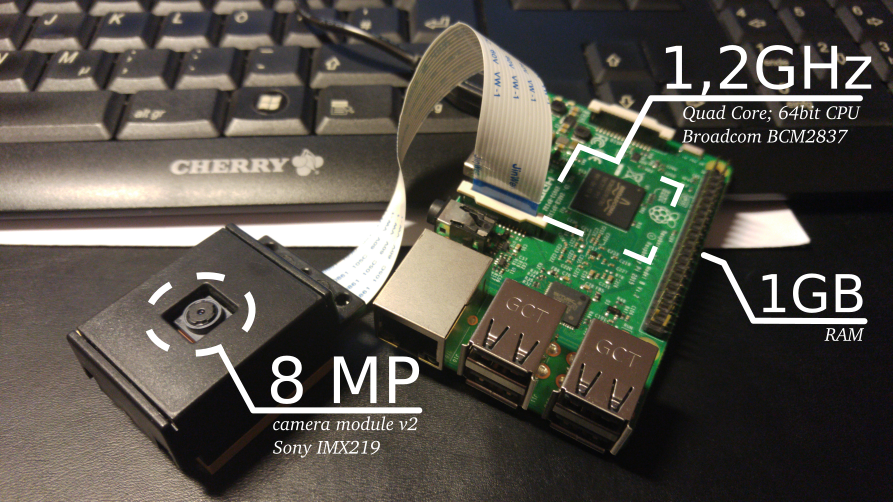
\includegraphics[width=0.9\textwidth]{raspi_camera}
	\caption{Raspberry Pi mit angeschlossenem Kameramodul}
\end{figure}

\subsection{Vorbereitung}
Bevor eine Klassifizierung durch das KNN stattfinden kann, müssen aus dem aufgenommenen Bild alle Gesichter extrahiert und auf einen gemeinsamen Standard normalisiert werden.

\subsubsection{Aufnahme des Kamerabildes}
Die Kamera liefert einen kontinuierlichen Datenstrom von Farbbildern mit einer Auflösung von bis zu \(3280 \times 2464\) Pixeln.\cite{raspberrypi:camera} Dieses Bild wird als Pixelmatrix gespeichert und weiter verarbeitet. Dabei wird das nächste Bild erst erfasst, wenn alle Gesichter im aktuellen Bild erkannt und ausgewertet wurden.

\subsubsection{Bildverarbeitung}
OpenCV speichert Bilder als zweidimensionale Matrizen. Die Anzahl der Spalten und Zeilen entsprechen dabei der Breite und Höhe des Bildes. Bei Graustufenbildern werden in der Matrix die Grauwerte gespeichert. In Farbbilder mit RGB-Farbsystem wird zu jedem Pixel ein Tripel mit Blau-, Grün- und Rotwert gespeichert.

\[
A =
\begin{pmatrix}
(B, G, R)_{00} & (B, G, R)_{01} & (B, G, R)_{02} \\
(B, G, R)_{10} & (B, G, R)_{11} & (B, G, R)_{12} \\
(B, G, R)_{20} & (B, G, R)_{21} & (B, G, R)_{22} \\
\end{pmatrix}
\text{Bildmatrix der Größe \(3 \times 3\)}
\]

Die folgenden Verfahren (\ref{sec:haar} und \ref{sec:lbp}) verwenden \textit{Faltungsmatrizen}. Dabei handelt es sich um Matrizen mit ungerader Kantenlänge, welche an jeder Position der Bildmatrix angewendet werden. Dazu wird die Faltungsmatrix pixelweise auf der Bildmatrix verschoben und für den jeweiligen Pixel werden Rechenoperationen durchgeführt.

\subsubsection{Graustufenumwandlung}
Für den Gesichtsausdruck ist nur die Struktur des Gesichts und nicht die Farbe wichtig. Aus diesem Grund wird die Datenmenge des Bildes auf die Grauwertinformationen reduziert. Dazu wird die Funktion \lstinline{cv2.cvtColor()} \cite{opencv:cvtcolor} mit dem Parameter \lstinline{cv2.COLOR_BGR2GRAY} verwendet. Sie berechnet einen Grauwert \(Y\) zu jedem Farbwert \((R, G, B)\):

\[Y = 0,299 \cdot R + 0.587 \cdot G + 0.144 \cdot B\]

Die Gewichtung der verschiedenen Farbkanäle entspricht der Empfindung des menschlichen Auges.\cite{wikipedia:grauwert}
% weiteres zur Kontrastanpassung durch Alphakorrektur

\subsubsection{Gesichtserkennung mit Haar Kaskaden}
\label{sec:haar}
Ein effizienter Algorithmus zur Gesichtserkennung in einem Bild mit Hilfe von Haar Features wurde von Paul Viola und Michael Jones 2001 veröffentlicht.\cite{violajones:paper} Dabei werden über das Grauwertbild Faltungsmatrizen verschoben. Die Faltungsmatrizen entprechen Haar Features und bestehen aus schwarzen, sowie weißen Bereichen. An jeder Position werden alle Grauwerte im schwarzen Bereich aufsummiert und anschließend von der Summer der Grauwerte im weißen Bereich abgezogen. Daraus entsteht eine Differenz, welche angibt, wie stark das jeweilige Feature ausgeprägt ist. Sind die beiden Bereiche sehr ähnlich, liegen die Summen in der gleichen Größenordnung und die Differenz ist folglich klein. Wenn die Bereiche dem Muster des Features folgen, unterscheiden sich die Summen stark voneinander und damit wird der Betrag der Differenz groß. Um möglichst alle Größen der Merkmale abzudecken, die ein Feature beschreibt, werden sie für den gesamten Prozess auf verschiedene Größen skaliert.

\begin{figure}
	\centering
	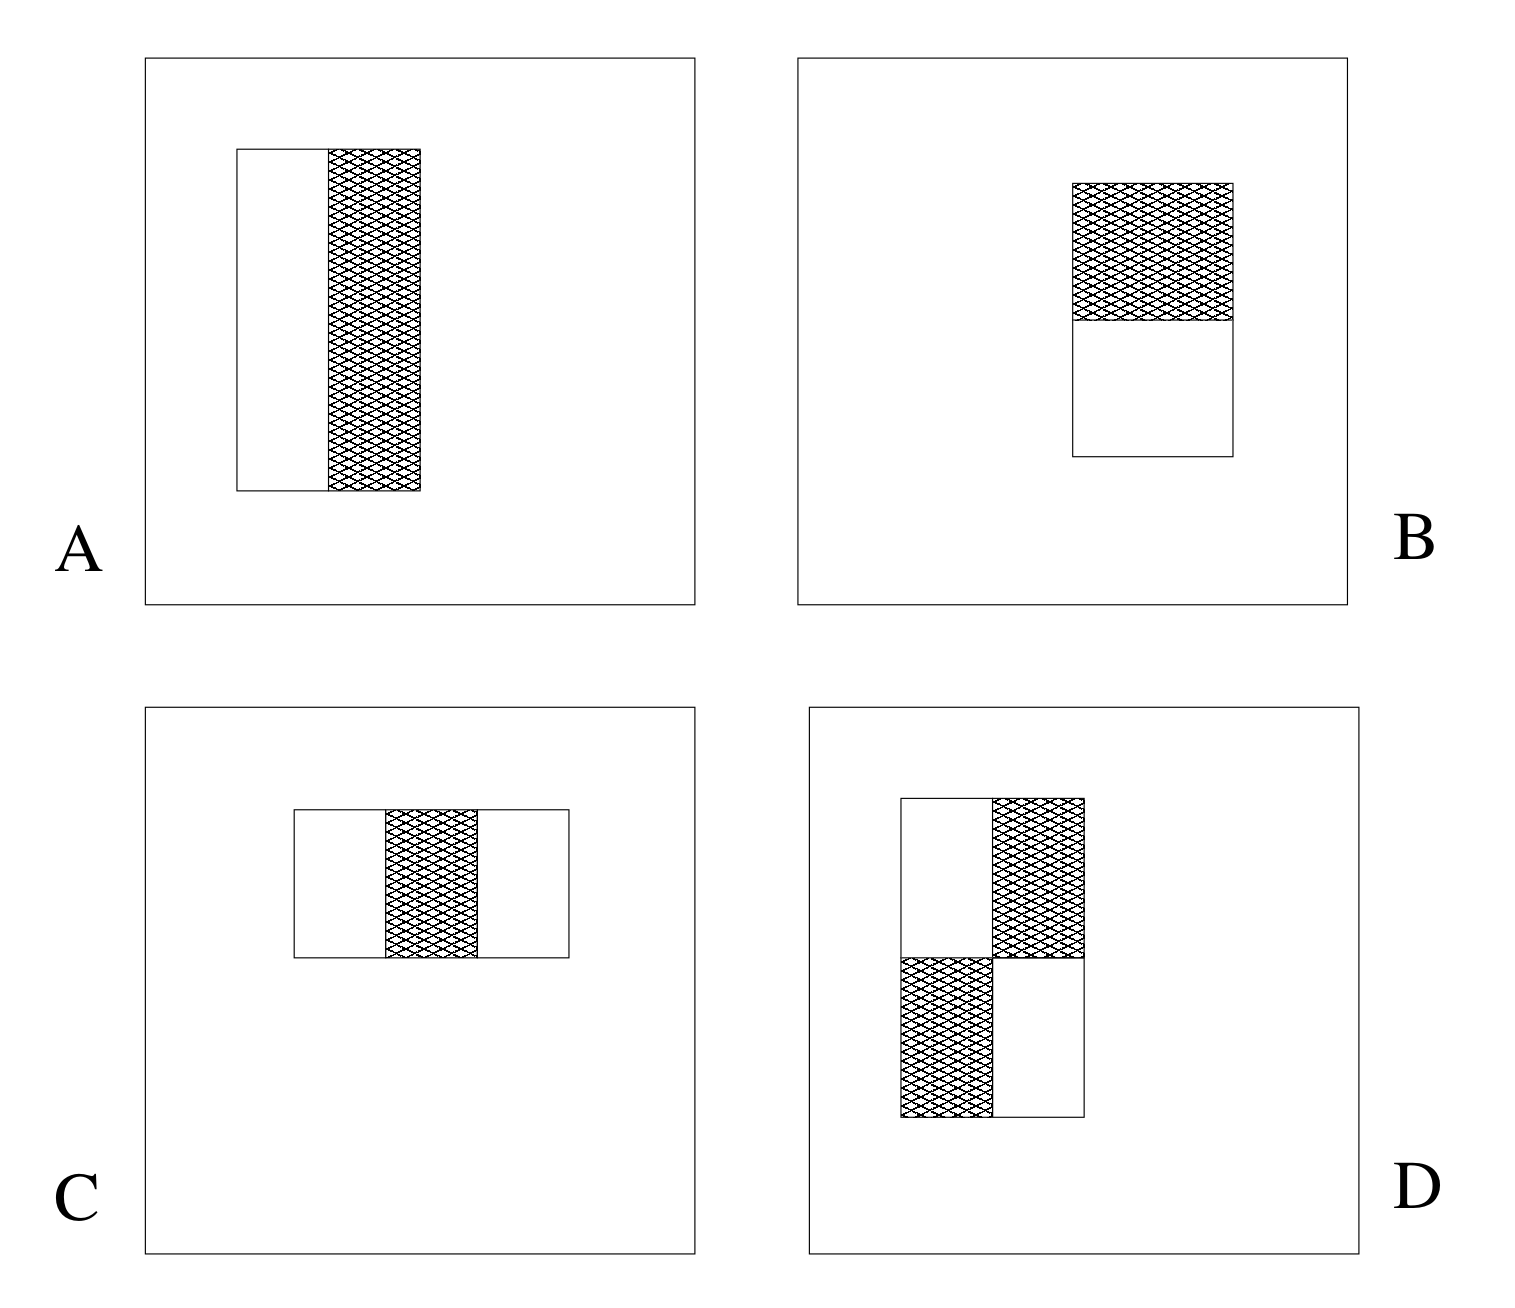
\includegraphics[width=0.5\textwidth]{haar_features}
	\caption{Haar Features\cite{violajones:paper}}
\end{figure}

Die so errechneten Mengen der verschiedenen Features werden mit dem Machine Learning Verfahren \enquote{AdaBoost} in relevante und unrelevante Features zum Erkennen von Gesichtern sortiert. Kombiniert bilden viele schwache Klassifizierer dann einen starken, welcher verwendet wird, um neue Gesichter zu erkennen. Das Berechnen der vielen Features für jedes Gesicht ist rechenaufwändig. Deshalb werden Regionen des Bildes verworfen auf welche die wichtigsten Features nicht zutreffen, um Bereiche die das Gesicht eher enthalten gründlicher Untersuchen zu können.

\subsubsection{Skalierung}
Um unterschiedliche Entfernungen der Gesichter von der Kamera zu kompensieren, werden die erkannten Gesichter auf eine festgelegte Größe von \(100 \times 100\) Pixel skaliert. Diese Bildgröße beinhaltet ausreichend viele Details und ermöglicht eine schnelle Verarbeitung. Sie wurde experimentell bestimmt und ist ein Kompromiss. Dabei wurden die notwendige Pixelanzahl für außreichend Details und geringe Speichernutzung, die Blockgröße des LBP und die Neuronenanzahl des KNN berücksichtigt.

\subsection{Local Binary Pattern}
\label{sec:lbp}

Das \textit{Local Binary Pattern} Verfahren ist eine statistische Auswertung des Bildes welches die Datenmenge stark reduziert. Dabei behält es die Kanten als wichtigste Information der Gesichtszüge bei.

Der folgende Algorithmus nutzt einen \(3 \times 3\) Ausschnitt, welcher an jede Position des Bildes verschoben wird. Dort werden jeweils alle äußeren Pixel mit dem mittleren verglichen. Ist der Grauwert des äußeren Pixels größer (heller), wird dieser auf 1 (weiß), ansonsten auf 0 (schwarz) gesetzt. Das zugehörige Pattern entsteht aus diesen Werten beginnend mit der linken oberen Ecke im Uhrzeigersinn gelesen. In Abbildung \ref{fig:lbp_pattern} ist eine Faltungmatrix dargestellt, deren Local Binary Pattern \((01100000)_{2}\) entspricht.

\begin{figure}
	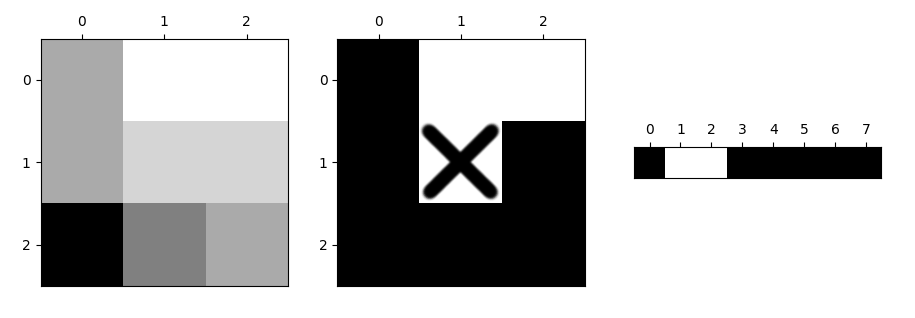
\includegraphics[width=\textwidth]{lbp_pattern}
	\caption{ \(3 \times 3\) Ausschnitt aus dem Grauwertbild, nach dem Vergleichen und als Pattern \((01100000)_{2}\) in grafischer Darstellung}
	\label{fig:lbp_pattern}
\end{figure}

\begin{center}
	\begin{struktogramm}(130, 70)[Local Binary Pattern]
		\assign%
		{
			\begin{declaration}[]
				\description{\(coordinates\)}{Liste der Koordinaten als Tupel}
				\description{\(matrix\)}{\(3 \times 3\) Matrix der Grauwerte des Kernels}
				\description{\(pattern\)}{Liste der Binären Vergleichsergebnisse}
			\end{declaration}
		}
		\assign{\(coordinates \gets  (0, 0),  (0, 1),  (0,2), (1, 2), (2, 2), (2, 1), (2, 0) , (1, 0) \)}
		
		
		\forallin{\(\forall coordinate\in coordinates\)}
		\ifthenelse{4}{4}{\(matrix[coordinate] > matrix[(1, 1)]\)}{\sTrue}{\sFalse}%
		\assign{\(1\) zu \(pattern\) hinzufügen}
		\change
		\assign{\(0\) zu \(pattern\) hinzufügen}
		\ifend
		\forallinend
	\end{struktogramm}
\end{center}


\subsubsection{Uniforme Pattern}

Als uniforme Pattern werden alle Pattern bezeichnet, die höchstens zwei Übergänge von 0 zu 1 oder 1 zu 0 enthalten.\cite{wikipedia:lbp}

Deshalb ist zum Beispiel \((00000101)_{2} = (5)_{10}\) kein uniformes Pattern, \((01100000)_{2} = (96)_{10}\) aber schon. Bei einer 8-bit Zahl ergeben sich 58 uniforme Pattern, welche in der folgenden Tabelle mit ihrer Binärdarstellung aufgeführt sind.

\medskip

\begin{tabular}{ | r r | r r | r r | }
	\hline
	\((0)_{10}\) & \((00000000)_{2}\) & \((62)_{10}\) & \((00111110)_{2}\) & \((207)_{10}\) & \((11001111)_{2}\) \\
	\((1)_{10}\) & \((00000001)_{2}\) & \((63)_{10}\) & \((00111111)_{2}\) & \((223)_{10}\) & \((11011111)_{2}\) \\
	\((2)_{10}\) & \((00000010)_{2}\) & \((64)_{10}\) & \((01000000)_{2}\) & \((224)_{10}\) & \((11100000)_{2}\) \\
	\((3)_{10}\) & \((00000011)_{2}\) & \((96)_{10}\) & \((01100000)_{2}\) & \((225)_{10}\) & \((11100001)_{2}\) \\
	\((4)_{10}\) & \((00000100)_{2}\) & \((112)_{10}\) & \((01110000)_{2}\) & \((227)_{10}\) & \((11100011)_{2}\) \\
	\((6)_{10}\) & \((00000110)_{2}\) & \((120)_{10}\) & \((01111000)_{2}\) & \((231)_{10}\) & \((11100111)_{2}\) \\
	\((7)_{10}\) & \((00000111)_{2}\) & \((124)_{10}\) & \((01111100)_{2}\) & \((239)_{10}\) & \((11101111)_{2}\) \\
	\((8)_{10}\) & \((00001000)_{2}\) & \((126)_{10}\) & \((01111110)_{2}\) & \((240)_{10}\) & \((11110000)_{2}\) \\
	\((12)_{10}\) & \((00001100)_{2}\) & \((127)_{10}\) & \((01111111)_{2}\) & \((241)_{10}\) & \((11110001)_{2}\) \\
	\((14)_{10}\) & \((00001110)_{2}\) & \((128)_{10}\) & \((10000000)_{2}\) & \((243)_{10}\) & \((11110011)_{2}\) \\
	\((15)_{10}\) & \((00001111)_{2}\) & \((129)_{10}\) & \((10000001)_{2}\) & \((247)_{10}\) & \((11110111)_{2}\) \\
	\((16)_{10}\) & \((00010000)_{2}\) & \((131)_{10}\) & \((10000011)_{2}\) & \((248)_{10}\) & \((11111000)_{2}\) \\
	\((24)_{10}\) & \((00011000)_{2}\) & \((135)_{10}\) & \((10000111)_{2}\) & \((249)_{10}\) & \((11111001)_{2}\) \\
	\((28)_{10}\) & \((00011100)_{2}\) & \((143)_{10}\) & \((10001111)_{2}\) & \((251)_{10}\) & \((11111011)_{2}\) \\
	\((30)_{10}\) & \((00011110)_{2}\) & \((159)_{10}\) & \((10011111)_{2}\) & \((252)_{10}\) & \((11111100)_{2}\) \\
	\((31)_{10}\) & \((00011111)_{2}\) & \((191)_{10}\) & \((10111111)_{2}\) & \((253)_{10}\) & \((11111101)_{2}\) \\
	\((32)_{10}\) & \((00100000)_{2}\) & \((192)_{10}\) & \((11000000)_{2}\) & 	\((254)_{10}\) & \((11111110)_{2}\) \\
	\((48)_{10}\) & \((00110000)_{2}\) & \((193)_{10}\) & \((11000001)_{2}\) & 	\((255)_{10}\) & \((11111111)_{2}\) \\
	\((56)_{10}\) & \((00111000)_{2}\) & \((195)_{10}\) & \((11000011)_{2}\) & & \\
	\((60)_{10}\) & \((00111100)_{2}\) & \((199)_{10}\) & \((11000111)_{2}\) & & \\
	\hline
\end{tabular}
\bigskip

 Diese Pattern stellen Kanten dar, während alle nicht uniformen Pattern eher weiche Übergänge beschreiben.

\subsubsection{Patternhäufigkeit}
\label{sec:patternhaufigkeit}

Um eine das Gesicht repräsentierende Statistik zu erhalten, wird das Bild in quadratische Blöcke mit einer festgelegten Seitenlänge unterteilt. Bei einer Blockgröße von beispielsweise 25 Pixeln und einer Bildgröße von \(100 \times 100\) Pixel ergibt das \(\frac{100}{25} \cdot \frac{100}{25} = 4 \cdot 4 = 16\) Blöcke. Für jeden dieser Blöcke wird gezählt, wie viele Pattern jeder Art darin vorkommen. Diese Häufigkeiten werden in einer Liste gespeichert, wobei Index 0 bis 57 den jeweiligen Pattern zugeordnet und in Index 58 alle nicht uniformen Pattern gezählt werden.

\begin{figure}
	\centering
	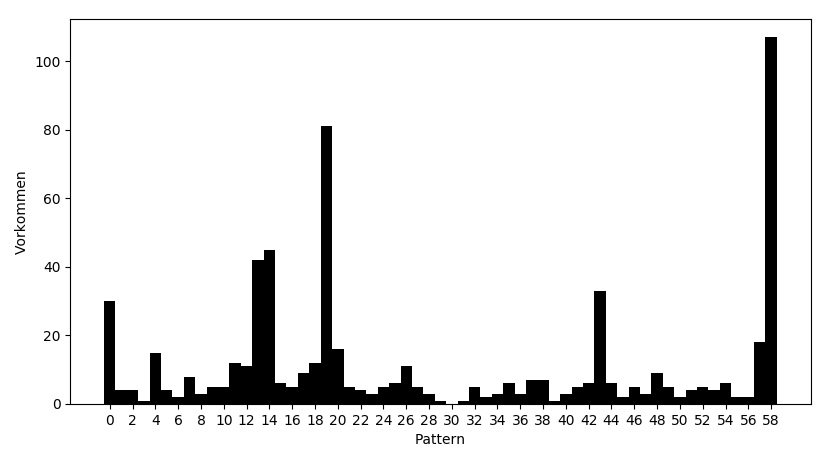
\includegraphics[width=\textwidth]{lbp_histogram_single}
	\caption{Absolute Häufigkeitsverteilung der Pattern im ersten Block (umrahmt) als Histogramm}
	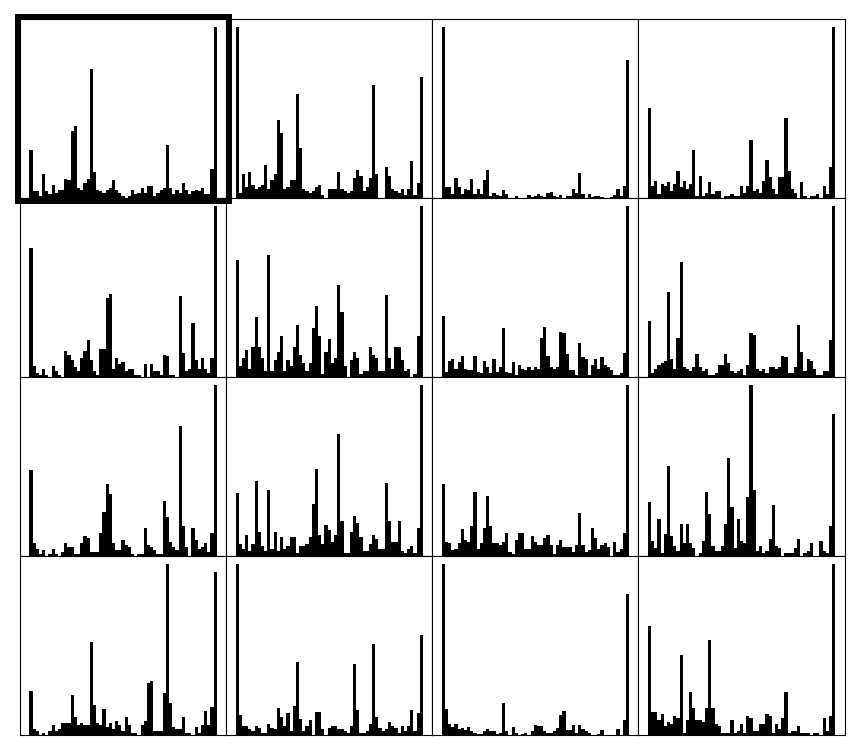
\includegraphics[width=0.9\textwidth]{lbp_histograms}
	\caption{Histogramme für alle 16 Blöcke des Bildes}
\end{figure}

\newpage

Durch dieses Vorgehen wird eine Häufigkeitsverteilung erstellt, die verschiedene Kantenarten erfasst und andere (nicht uniforme) Übergänge als ein Kriterium vereinfacht und somit die Anzahl der Klassen von 256 auf 59 reduziert. Während die Häufigkeiten die Merkmale des Blocks beschreiben, ist der Block an sich für die Speicherung des Ortes wo dieses Merkmal auftritt zuständig. Deshalb werden im letzten Schritt alle Häufigkeiten der Blöcke in einer festgelegten Reihenfolge zum Eingabevektor für das künstliche Neuronale Netz in \ref{sec:auswertung} zusammengefügt.
\[X =
\begin{pmatrix}
	H_{Block 0, Pattern 0} \\
	\vdots \\
	H_{Block 0, Pattern 58} \\
	\vdots \\
	H_{Block 15, Pattern 0} \\
	\vdots \\
	H_{Block 15, Pattern 58} \\
\end{pmatrix} \]


\subsection{Auswertung}
\label{sec:auswertung}
Aus der statistischen Repräsentation des Gesichts soll jetzt mit Hilfe eines KNNs eine Relation zu der jeweilig vorliegenden Emotion hergestellt werden. Dabei wird dem Eingabevektor aus \ref{sec:patternhaufigkeit} ein 7-dimensionaler Zielvektor \(Y\) zugeordnet, der überall außer bei der richtigen Emotion, wo der Wert 1 steht, eine 0 enthält. Mit überwachtem Lernen wird das Netz auf die Verbindung zwischen den beiden trainiert.

\subsubsection{FeedForward KNNs}
FeedForward Netze sind künstliche neuronale Netze und bestehen aus einer Eingabeschicht, mehreren versteckten Verarbeitungsschichten und einer Ausgabeschicht. Die jeweilige Schicht besteht aus mehreren Neuronen. Jedes Neuron ist mit allen anderen Neuron der folgenden Schicht über Kanten verbunden. Zwischen einer Schicht mit 4 Neuronen und einer mit 3 Neuronen existieren also \(4 \cdot 3 = 12\) Kanten.

Um ein Ergebnis aus dem Netz zu erhalten, ist eine Eingabe nötig. Diese ist der vorher auf Werte von 0  bis 1 normalisierte Eingabevektor \(X\). Die im Vektor enthaltenen Zahlen entsprechen dabei den Werten der Neuronen der Eingabeschicht.

\subsubsection{Gewichte}
Die Gewichte repräsentieren die Stärke der Verbindung (Kanten) zwischen zwei Neuronen \(i\) und \(j\) und speichern das gelernte Wissen. Diese Verbindung wirkt somit  verstärkend oder hemmend auf die Aktivität des Neurons \(j\).

Die Eingaben sind die Produkte aus den Aktivierungen \(a_{i},...,a_{i_{n}}\) aller vorherigen Neuronen \(i_{1},...,i_{n}\) und den Gewichten \(w_{ji_{1}},...,w_{ji_{n}}\) die diese Neuronen mit \(j\) verbinden, zur Netzeingabe \(z_{j}\) aufsummiert. \cite[S.~37]{dkriesel:paper}
\[z_{j} = \sum_{i = 1}^{n} w_{ji} \cdot a_{i}\]

Aus den Aktivierungen der Neuronen einer Schicht als n-dimensionaler Vektor \(A\) und einer Gewichtsmatrix \(W\) mit der Größe \(m \times n\) berechnet sich der m-dimensionale Eingabevektor \(Z\) der nächsten Schicht.
\[Z = W \cdot A\]
\[
\begin{pmatrix}
z_{1} \\
\vdots \\
z_{m}
\end{pmatrix}
 = 
\begin{pmatrix}
w_{11} & \dots & w_{1n} \\
\vdots & \ddots & \vdots \\
w_{m1} & \dots & w_{mn}
\end{pmatrix}
 \cdot
\begin{pmatrix}
a_{1} \\
\vdots \\
a_{n}
\end{pmatrix} 
=
\begin{pmatrix}
w_{11} \cdot a_{1} +\dots + w_{1n} \cdot a_{n} \\
\vdots \\
w_{m1} \cdot a_{1} + \dots + w_{mn} \cdot a_{n}
\end{pmatrix} 
\]

Die Python Bibliothek \textit{numpy} ermöglicht es für die Matrixmultiplikation mehrere Kerne parallel zu nutzen. Da die Mikroprozessoren für Matrixberechnungen optimiert sind, werden die Formeln in Matrixdarstellungen umgewandelt.

\subsubsection{Bias}
Die Aktivierung eines Neurons ist abhängig von den Aktivitäten der Neuronen in der vorherigen Schicht. Um zu modellieren, dass manche Neuronen generell verschiedene Aktivitätsgrade besitzen, fügt man einen Schwellwert ein, der steuert ab wann ein Neuron zu feuern anfängt. Es besteht die Möglichkeit diesen Schwellwert von der Netzeingabe \(z_{j}\) abzuziehen. Damit der Schwellwert mit dem gleichen Verfahren, wie die Gewichte beim Training anpassen werden kann, wird er als Gewicht eines unabhängigen, zusätzlichen Neurons in der vorherigen Schicht implementiert. Dieses Biasneuron hat immer die Ausgabe \(a_{bias} = 1\). Der Schwellwert ist also nur vom Wert des Gewichts vom Biasneuron zum jeweiligen Neuron abhängig. Da alle Neuronen einer Schicht mit allen Neuronen der vorherigen Schicht verbunden sind, reicht ein Biasneuron pro Schicht um für die gesamte nächste Schicht Schwellwerte bereitzustellen.

\subsubsection{Aktivierungsfunktion}
Die Aktivierungsfunktion \(\phi\) berechnet aus der Netzeingabe \(z\) die Aktivierung \(a\). 
\[a = \phi(z) \]
Natürliche Neuronen feuern nicht über einen bestimmten Maximalwert hinaus.  Deshalb bildet die Aktivierungsfunktion Zahlenwerte in einem festen Bereich ab.

Häufig wird die Sigmoid Funktion verwendet, da sie die Eingabe auf Werte von 0 bis 1 normalisiert. Sie ist im Bereich um 0 sehr sensibel und normalisiert stark bei Betragsmäßig großen Eingaben. Eine weitere Bedingung an die Aktivierungsfunktion ist die Differenzierbarkeit, welche für die Gewichtsanpassung in \ref{training} nötig ist.
\[\phi(z) = sigmoid(z) = \frac{1}{1 + e^{-z}}\]

\begin{figure}
	\centering
	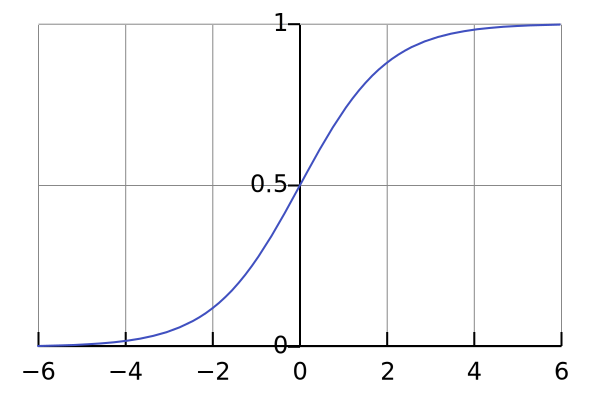
\includegraphics[width=0.5\textwidth]{Logistic-curve}
	\caption{Sigmoid Funktion\cite{img:wikipedia:sigmoid}}
\end{figure}

\subsubsection{Training}
\label{training}

Beim Trainieren eines künstlichen neuronalen Netzes werden nacheinander Bilder aus einem Trainingsset zu denen das gewünschte Ergebnis bekannt ist ins Netz eingegeben. Das gleiche Trainingsset kann in mehreren Durchläufen (Epochen) wiederholt werden, um im Gradientensbstiegsverfahren den Fehler des Netzes zu minimieren. Dabei muss die Reihenfolge immer zufällig sein, um das Lernen der Abfolge von Eingaben zu vermeiden.

Nach dem Training wird mit Testdaten überprüft, wie gut das Netz abstahiert hat, indem man dem Netz noch unbekannte Gesichter verwendet. Dabei werden die Gewichte nicht angepasst, sondern nur das Resultat des Netzes ausgewertet. Als Testscore speichert man, wie viele der Trainingsdaten richtig klassifiziert wurden, wobei das Neuron mit der größten Ausgabe der vom Netz erkannten Emotion entspricht. Wenn der Fehler beim Training zwar gering ist, der Score beim Testen aber schlecht, wurde das Netz mit zu vielen Epochen übertrainiert und kann deshalb zwar die bekannten Gesichter erkennen, verfügt aber nicht über allgemeines Wissen, welches für unbekannte Gesichter nötig ist.

\paragraph{Fehler}
Um nach Eingabe eines Trainingsbeispiels in das KNN die Gewichte so anpassen zu können, dass sie das Resultat des Netzes verbessern, muss der Fehler des jeweiligen Beispiels gemessen werden. Er ergibt sich als Differenz aus dem Zielvektor \(Y\) und dem Ausgabevektor \(A\).
\[E = Y - A\]

\paragraph{Backpropagation}
Bevor die Gewichte angepasst werden, muss der Fehler für jedes Neuron berechnet werden. Dies ist bis jetzt nur in der Ausgabeschicht geschehen, wo eine direkte Berechnung möglich ist. Die Backpropagation führt die Fehler der Ausgabeschicht in die vorherigen Schichten zurück. Dabei wird der Fehler eines Neurons \(j\) so auf die mit ihm verbundenen Neuronen \(i_{1}, \dots, i_{n}\) zurückgeführt, dass die durch stärkere Gewichte verbundenen, und damit mehr am Fehler beteiligten, Neuronen einen größeren Anteil am Fehler erhalten. Wenn der Fehler mit dem verbindenden Gewicht multipliziert wird, ist diese Proportionalität hergestellt. Als Matrixmultiplikation berechnet sich der Fehlervektor \(E_{i}\) aus dem Fehlervektor \(E_{j}\) und den verbindenden Gewichten \(w_{ji}\) wie folgt:

\[E_{i} = W^T \cdot E_{j}\]
\[
\begin{pmatrix}
	e_{i_{1}} \\
	\vdots \\
	e_{i_{n}}
\end{pmatrix}
=
\begin{pmatrix}
w_{11} & \dots & w_{m1} \\
\vdots & \ddots & \vdots \\
w_{1n} & \dots & w_{mn}
\end{pmatrix}
\cdot
\begin{pmatrix}
e_{j_{1}} \\
\vdots \\
e_{j_{m}}
\end{pmatrix}
\]

Im Gegensatz zur Vorwärtsberechnung, bei der die Summe aller zu  \(j_{1}\) führenden Gewichte multipliziert mit allen \(a_{i_{1}},\dots,a_{i_{m}}\) gesucht wird, multipliziert man bei der Fehlerberechnung die Summe aller zu \(e_{i_{1}}\) führenden Gewichte  mit allen \(e_{j_{1}},\dots,e_{j_{m}}\). Dazu nutzt man die transponierte Gewichtsmatrix \(W^T\).

Der so erhaltene Fehlervektor kann nach dem gleichen Prinzip für alle versteckte Schichten berechnet werden.

\paragraph{Gradientenabstiegsverfahren}
Die Gewichte können nicht so angepasst werden, dass der resultierende Fehler 0 wird. Deshalb wird versucht in mehreren Schritten die Gewichte so zu verändern, dass der Fehler gegen 0 konvergiert.

Der Gesamtfehler ist die Summe  der Einzelfehler. Damit sich bei der Aufsummierung positive und negative Fehler nicht aufheben, wird die  quadratische Kostenfunktion verwendet. Sie berechnet den Kostenvektor wie folgt:
\[C = (A - Y)^2\]
Im Gegensatz zum Absolutwert weist diese Funktion einen immer kleiner werdenden Gradienten auf, je weiter man sich einem Minimum nährt.

Um zu wissen, ob ein Gewicht \(w\) zu groß oder zu klein ist, betrachtet man die partielle Ableitung von \(\frac{\partial c}{\partial w}\). Sie gibt an, um wie viel sich \(c\) bei einer kleinen Veränderung von \(w\) ändert  und  ist damit der Anstieg der Kostenfunktion.

Durch Ableiten der Kostenfunktion und der Aktivierungsfunktion, kann unter Anwendung der Kettenregel  \(\frac{\partial c}{\partial w}\)  berechnet werden. Ist dieser Anstieg positiv, muss das Gewicht verringert werden, um die Kosten zu senken. Bei einem negativen Wert, minimiert eine Erhöhung des Gewichts die Kosten. Die Anpassung muss also in die entgegengesetzte Richtung zum Anstieg der Kostenfunktion stattfinden. Bei einer proportionalen Anpassung ist die Schrittweite abhängig vom Anstieg. Die Kostenfunktion weist eine Parabelform auf. Nährt man sich dem Minimum, wird der Anstieg kleiner. Deshalb ist die Schrittweite zu Beginn groß und sinkt allmählich. So wird das Überspringen des Minimums durch zu große Schritte verhindert.
\[w' = w - \eta \frac{\partial c}{\partial w}\]
Als Proportionalitätsfaktor wird zusätzlich die Lernrate \(\eta\) verwendet um die Schrittweite zu skalieren. Sie sollte dabei weder zu klein noch zu groß gewählt werden, da das Netz ansonsten zu lange zum Trainieren braucht, oder aber das gefundene Minimum der Kostenfunktion übersprungen wird.

\paragraph{Trainingsverfahren}
Werden die Gewichte nach jedem Trainingsbeispiel angepasst, sprich man vom Online-Lernen. Es betrachtet beim Wählen des nächsten Schrittes nur eine einzelne Eingabe. 

Beim Offline-Lernen werden zunächst alle Trainingsbeispiele durchgegangen und dann die durchschnittliche Gewichtsanpassung ermittelt und angewendet. Dies ist wesentlich zeitaufwändiger, berücksichtigt aber die optimale Veränderung für alle Trainingseingaben. 

\paragraph{Gewichtsinitialisierung}
Zu Beginn des Trainings werden alle Gewichte mit zufälligen Werten initialisiert. Die Initialisierung ist dafür verantwortlich, welche Ausgangswerte das Netz verwendet.

Durch eine ungünstige Ausgangskonfiguration des Netzes kommt es vor, dass Trainingsdurchläufe negativ beeinflusst werden. Es wird dadurch nur ein lokales Minimum der Kostenfunktion gefunden. Um optimale Ausgangswerte für eine Netzkonfiguration zu finden, sollte man mehrere Trainings mit unterschiedlichen Belegungen der Gewichtswerte durchführen.
Um zu erreichen, dass die Netzeingabe \(z\) in einem definierten Bereich liegt, kann man die Gewichtsinitialisierung abhängig von der Anzahl \(n\) der Neuronen der vorherigen Schicht machen.
\[-\frac{1}{\sqrt{n}} < w < \frac{1}{\sqrt{n}}\]

\subsection{Trainingsdaten}
Um das künstliche neuronale Netz zu trainieren, wird eine große Menge nach Emotionen klassifizierter Bilder von Gesichtsausdrücken benötigt. Diese Bilder sollten ein großes Spektrum unterschiedlicher Gesichtstypen abdecken,  damit das trainierte Netz unabhängig von  Alter, Hautfarbe, Geschlecht oder Frisur einsetzbar ist. In den drei verwendeten Datenbanken wurden Personen angewiesen eine bestimmte Emotion zu zeigen.

Aus der JAFFE Datenbank werden 183, aus COHN 326 und aus KDEF 840 Bilder verwendet. Idealerweise sollten 70\% der verfügbaren Beispiele zum Training und 30\% zum Testen genutzt werden. Aufgrund der relativ wenigen Daten wurden die ersten 150 Bilder jeder Emotion zum Trainieren verwendet und die Übrigen zum Testen genutzt. Dies beeinflusst die Testergebnisse, nutzt aber möglichst viele Trainingsdaten. Das Trennen von Trainings- und Testdaten ist wichtig, damit das Netz die Beispiele nicht auswendig lernt (overfitting), sondern allgemeine Strukturen erlernt.

Die Gesichter wurden mit der in \ref{sec:haar} beschriebenen Methode erkannt, auf \(100 \times 100\) Pixel skaliert und damit normiert. In einer Datenbank wird der Dateiname und der zugeordnete Emotionscode festgehalten. Die Emotionen sind in den genutzten Emotionsdatenbanken zu gleichen Teilen repräsentiert.  Allerdings wurden nicht alle Gesichter der Beispieldatensätze erkannt, wodurch es minimale Abweichungen in der Anzahl der einzelnen Emotionen gibt. Die Emotion \textit{verachtend} ist nur in der COHN Datenbank enthalten und deshalb mit 25 (statt 190 bis 250) Bildern unterrepräsentiert.

\begin{figure}[h]
	\centering
	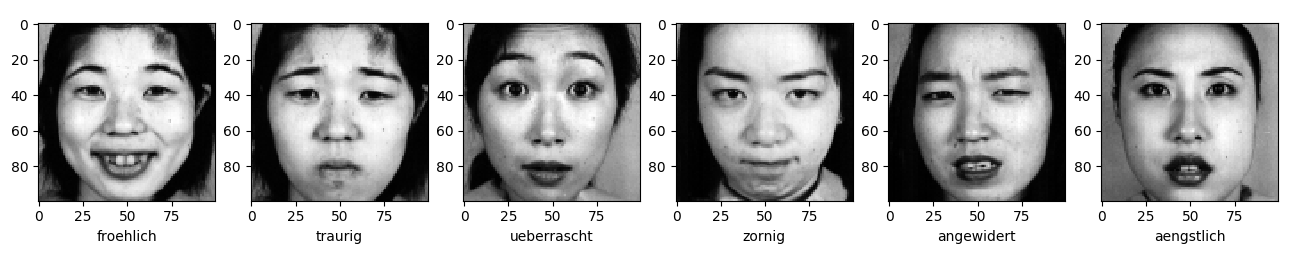
\includegraphics[width=0.85\textwidth]{jaffe_emotions}
	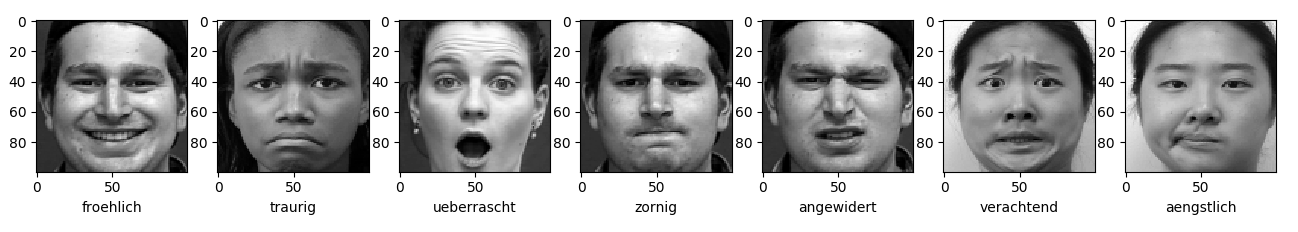
\includegraphics[width=1.0\textwidth]{cohn_emotions}
	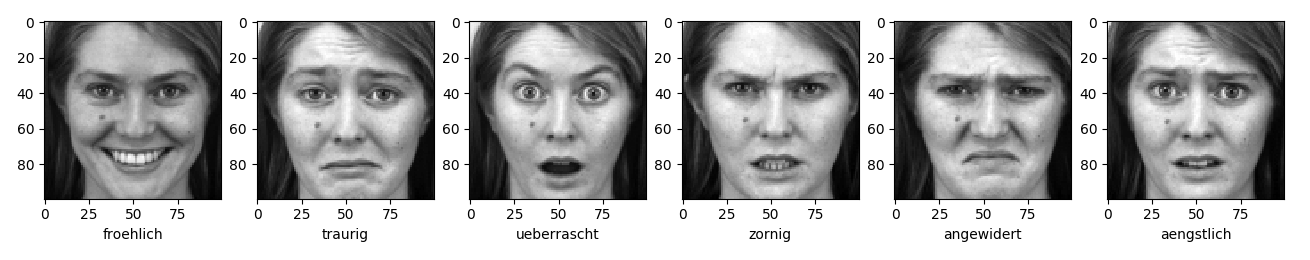
\includegraphics[width=0.85\textwidth]{kdef_emotions}
	\caption{Beispiele aus JAFFE\cite{db:jaffe}, COHN\cite{db:cohn1} und KDEF\cite{db:kdef}}
\end{figure}

\newpage
\section{Ergebnisse}
Die Lernrate, Blockgröße und Struktur der versteckten Schichten sind \textit{Hyperparameter}. Sie werden vorgegeben und empirisch ermittelt. Dabei muss immer ein Kompromiss zwischen höherer Genauigkeit und längeren Trainingszeiten gefunden werden.

Aus einer kleineren Blockgröße resultieren beispielsweise mehr Blöcke und damit aussagekräftigere statistische Daten. Die höhere Blockanzahl erfordert jedoch mehr Eingabeneuronen für das Netz. Daraus ergibt sich eine größere Menge an Gewichten in der Folgeschicht. 

Beim Lernen steigt mit zunehmender Gewichtsanzahl der Rechenaufwand. Daher muss eine Blockgröße gewählt werden, welche maximal groß ist um alle Details gerade noch zu beinhalten, jedoch gleichzeitig die Blockanzahl möglichst gering hält.

\begin{figure}[p]
	\centering
	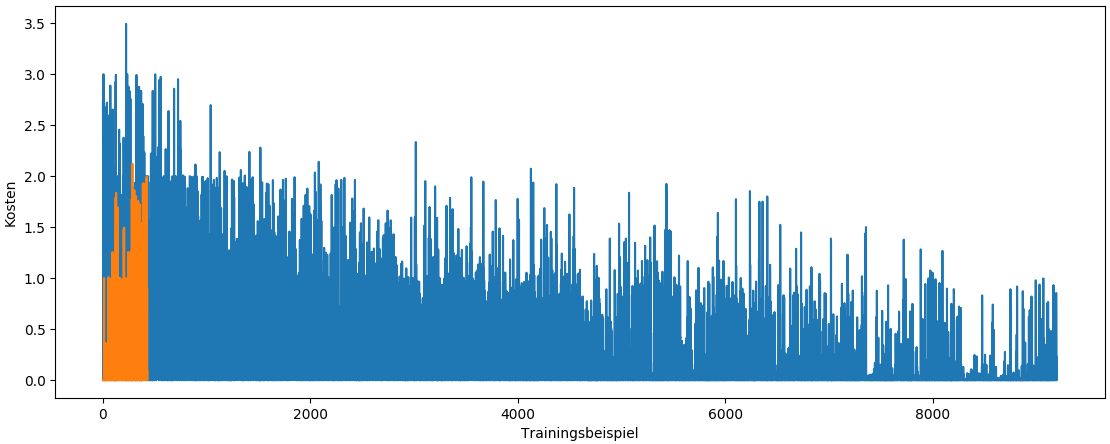
\includegraphics[width=1\textwidth]{82_score_costs}
	\caption{Kosten beim Training (blau) sowie beim Testen (orange)}
	\label{fig:costs_best_score}
\end{figure}

\begin{figure}[p]
	\centering
	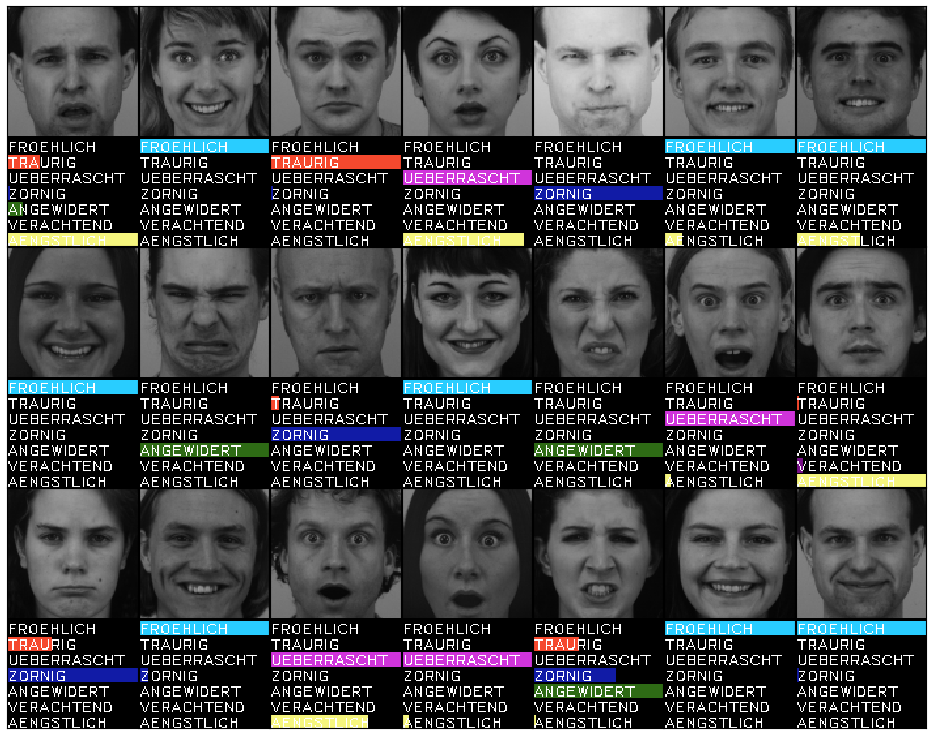
\includegraphics[width=1\textwidth]{detection_results_2}
	\caption{Erkannte Emotionen von Testdaten}
	\label{fig:emots_best_score}
\end{figure}

\begin{figure}[p]
	\centering
	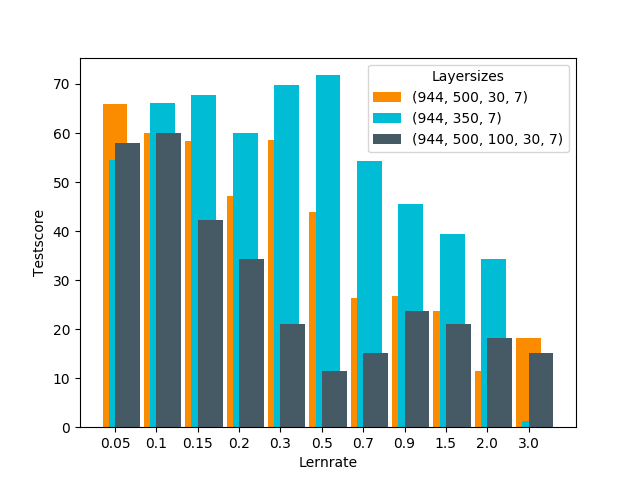
\includegraphics[width=1\textwidth]{learningrate_score}
	\caption{Testscores bei verschiedenen Lernraten für unterschiedliche Netzkonfigurationen (siehe Legende) mit Blockgröße 25}
	\label{fig:learningrate_score}
\end{figure}

Die beste Konfiguration erkannte 82,75\% der Testbilder richtig. Die Blockgröße ist 10, die Schichten sind (5900, 2000, 7) und die Lernrate beträgt 0.2. In Abbildung \ref{fig:costs_best_score} sieht man den Kostenverlauf während des Trainings über 10 Epochen (blau) und beim Testen (orange). Da die Kosten bis zum Ende mit Ausschlägen sinken, ist es wahrscheinlich, dass durch weitere Epochen Training noch ein geringerer Fehler zu erreichen wäre. In Abbildung \ref{fig:emots_best_score} sieht man die Emotionen, die das Netz in einem Auszug aus den Testdaten erkannt hat. Der Farbige Anteil des Balken gibt den Anteil des jeweiligen Ausgabeneurons an der höchsten Ausgabe an.

In Abbildung \ref{fig:learningrate_score} sind drei Netzkonfigurationen (orange, blau, schwarz) und deren Testergebnisse nach dem Trainieren mit Lernraten von \textit{0,05; 0,1; 0,15; 0,2; 0,5; 0,7; 0,9; 1,5; 2} und \textit{3} dargestellt. Die Netzkonfiguration mit den geringsten Schichten erzielte immer außer bei einer Lernrate von 0.05 die besten Ergebnisse. Ihre optimale Lernrate liegt bei 0.5, während diese Rate für die Konfiguration mit den meisten Schichten die schlechteste ist.

\subsection{Verbesserungen}
Mögliche Verbesserungen wären das Ausprobieren von weiteren Netzkonfigurationen mit Schichtanzahl und Schichtgröße. Die Blockgrößen des Local Binary Pattern Verfahrens und die Lernrate bieten auch noch weitere Testmöglichkeiten an. Außerdem würden größere Gesichtsdatenbanken mehr Testdaten ermöglichen und damit die ungleichmäßige Verteilung der Testbilder pro Emotion verhindern, sowie generell mehr Trainingsdaten bereitstellen.

Das Anpassen der Bildhelligkeit oder eine Erhöhung des Kontrasts vor der statistischen Verarbeitung könnten ebenfalls für bessere Ausgangsdaten sorgen.

Zuletzt ist die Beschränkung der Klassifizierung auf genau eine Emotion unrealistisch, da mehrere Emotionen überlagert ausgedrückt werden können. Diese Zweitemotionen werden aber immer als Fehler gewertet.

Das Lernverfahren kann zu einem Offline oder Mini-Batch Verfahren erweitert werden, was präzisere Schritte im Gradientenabstiegsverfahren ermöglicht. Außerdem könnte die Momentummethode eingesetzt werden, um gefundene lokale Minima zu verlassen und weiter nach dem globalen Minimum zu suchen.

\newpage
\nocite{db:cohn2}
\nocite{nnadl}
\nocite{nnsp}

\section{Anhang}
\printbibliography[heading=subbibintoc, keyword=book]
\printbibliography[heading=subbibintoc, type=online, title={Websites}]
\printbibliography[heading=subbibintoc, keyword=database, title={Datenbanken}]
\printbibliography[heading=subbibintoc, type=misc, title={Bild}]

\bigskip
\hrulefill

\textit{\small{Dieses Werk ist außer den durch Quellenverweis zitierten Fremdinhalten und Gesichtsdatenbanken unter einer Creative Commons Lizenz vom Typ Namensnennung - Weitergabe unter gleichen Bedingungen 4.0 International zugänglich. Um eine Kopie dieser Lizenz einzusehen, konsultieren Sie http://creativecommons.org/licenses/by-sa/4.0/ oder wenden Sie sich brieflich an Creative Commons, Postfach 1866, Mountain View, California, 94042, USA.}}

\bigskip
Der Quellcode, welcher für diese Arbeit entstand ist unter GPLv3 veröffentlicht: \url{https://github.com/hermlon/nnemotions}

\newpage
\paragraph{Selbstständigkeitserklärung}
Hiermit erkläre ich, dass ich die vorliegende Arbeit selbstständig und ohne unerlaubte fremde Hilfe angefertigt, keine anderen als die angegebenen Quellen und Hilfsmittel verwendet und die den verwendeten Quellen und Hilfsmitteln entnommenen Stellen als solche kenntlich gemacht habe.\cite{selbststaendigkeit}

\bigskip
\hfill
Halle (Saale)

\hfill
2018-06-07


\end{document}
